\section{What Reading the Binaries Shows}
\label{sec:findings}

% VALUE: reading the open and closed stacks' binaries shows the array idle while the device reads busy, per stack; the waits behind it are textbook false dependences that lowering reintroduces, placed on a grid of cause and granularity; the census measures how often they occur across a fixed population
Measuring the MLIR-AIR designs and reading FastFlowLM's binaries shows where the array idles although the device is busy (Section~\ref{subsec:losses}).
The waits behind the idle time are the textbook false dependences, which lowering to the CP's stream and to the cores' loops reintroduces, and we place each instance on a grid of cause and granularity (Section~\ref{subsec:grid}).
A census over a fixed population of streams from all three stacks counts how often they occur (Section~\ref{subsec:census}).
What each stack contributes differs: the MLIR-AIR instances are measured, FastFlowLM enters through one captured prefill and the census, and IRON through the census alone.

\subsection{The Idle Array}
\label{subsec:losses}

\begin{figure}[t]
    \centering
    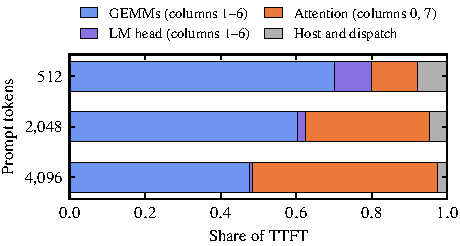
\includegraphics[width=\linewidth]{fig/busy.pdf}
    % VALUE: in the existing prefill, attention's share grows with prompt length, and each column group idles while the other computes
    \caption{Share of TTFT of the existing Llama-3.2-1B prefill by prompt length. Device-busy parts are each operator's time when dispatched alone, less the dispatch floor, summed over the prefill.}
    \label{fig:busy}
\end{figure}

\textbf{Column Groups in Prefill.}
% VALUE: the existing prefill issues one operator per command, so its column groups take turns; the device is busy almost all the time, but on one group at a time, and attention's growing share is time the GEMM columns sit idle
The existing prefill issues one operator per command, which amounts to about 1{,}500 commands for a 2{,}048-token prompt.
Figure~\ref{fig:busy} shows the resulting split of TTFT: device-busy time accounts for 92--97\% of it, and attention's share grows from 12\% to 49\% between 512 and 4{,}096 tokens.
Because the commands run in submission order, columns 1--6 idle while attention runs, and columns 0 and 7 idle while the GEMMs run, although neither group consumes the other's current work.
The device is thus busy almost all of the time, but on only one column group at a time.
% SOURCE: commands = 16 layers x chunks x 6 + 11 LM-head commands = 1,547 at 2,048 tokens (vault lab-prefill-census (1)).
% SOURCE: amd-npu e3acc8a prefill-e2/decomp.txt via figs/make_figs.py: busy = isolated time - dispatch floor = 92/95/97% of TTFT at 512/2k/4k; of TTFT, attention 12.2/32.9/49.1%, GEMMs 70.1/60.3/47.6%, LM head 9.7/2.1/0.8%.
% SOURCE: serial execution, the isolated busy times sum to at most TTFT (vault lab-prefill-device (4)); queued commands do not overlap (Section 3.1).

\textbf{Columns of One Operator.}
% VALUE: the same loss occurs inside one operator: the existing attention stream starts column 7 only after waiting on column 0, which costs a third of attention's device time
The existing attention stream issues column~7's inputs only after two synchronizations on column~0's key and value transfers, which complete when column~0 is about half done.
Alternating the two columns' segments, so that both columns start before the CP waits on either, reduces attention's device-busy time to $0.67\times$ that of the existing order at every chunk of a 2{,}048-token prompt, with bit-identical outputs.
Each column's half alone takes the same time within 1\%, so the difference comes from the CP's instruction order rather than from an imbalance of work.
Since attention's share grows with the prompt, this loss grows with it.
% SOURCE: decoded from the shipped a_32_4_0_0 stream, mid-stream synchronizations at ops 70, 75 (column 0) and 92, 97 (column 7); column 7's issue (ops 81-91) follows column 0's two mid-stream synchronizations (vault lab-prefill-overlap (4)).
% SOURCE: (alternated - F) / (existing - F) = 0.666-0.668 on 7 pairs, chunks 2-14 at 2,048 tokens; column 7 alone / column 0 alone = 0.994-1.010 (amd-npu 17f7ec3 ovl4/, vault lab-prefill-overlap (5)c); at absolute chunks 16-255: Qwen3-4B 0.66-0.68; Llama-3.2-1B 0.66 / 0.57 / 0.41 / 0.43 / 0.68 / 0.67 / 0.66, lower at its mid-range chunks (vault lab-agent-step (4)).

\textbf{Transfers in Decode.}
% VALUE: decode's per-token time grows linearly with context and attention becomes most of it; attention reads the KV cache at half the platform's read rate because the single-buffered KV loop serializes each block's transfer behind the previous block's compute, not because of the transfer or its placement
The existing decode design places attention's cores on columns 3 and 4 and reads the KV cache through those columns' two shim tiles.
Its time per token grows linearly with the context, within 0.2\% between 2{,}048 and 32{,}704 tokens, and attention's share of that time grows from 13\% to 70\% over the same range.
During attention, the design reads the KV cache at 51\% of the DRAM read cap measured in the same batch.
The transfer is not the limit: a build that streams 30{,}720 further positions with no further compute reads them at the two shim tiles' full rate, 88\% of the cap.
Nor is the CP's order the limit, since each layer issues the next projection's weights before it waits on the KV cache.
Instead, the design's KV loop is single-buffered, because its running maximum and accumulator live across blocks and MLIR-AIR's double-buffering transformation declines such loops, so each block's transfer waits for the compute on the previous block, which adds 41\% of the time per position.
Spreading attention over more columns would therefore gain little, since the transfer alone already reads near the cap.
% SOURCE: per-token time = 15.94 ms + 1.156 us x L, max residual 0.2% over L = 2,048-32,704 (Llama-3.2-1B, one 32k-window build, median of 3); 32 KiB per position / 1.156 us = 28.4 GB/s against a same-batch 8x2 cap of 55.2 GB/s; attention 13/23/37/54/70% of per-token time at 2k/4k/8k/16k/32k (vault lab-decode-long-context (5)).
% SOURCE: footprint from the build's npu.air.mlir: KV readback on shims 3 and 4, attention cores on columns 3 and 4 (vault lab-decode-long-context (6)).
% SOURCE: bytes-only discriminator: ELF window 32,768 vs 2,048 at the same small L, 20.81 ms / 30,720 positions = 0.677 us = 48.4 GB/s = 88% of the 55.2 GB/s cap and 104% of the two-shim probe; serialized compute 1.156 - 0.677 = 0.478 us = 41% of the per-position time (vault lab-decode-long-context (7)).
% SOURCE: per layer, the QKV weight streams are awaited, then the KV readbacks start, and the next projection's weight streams are issued before any KV await; weight progress during attention is bounded by buffering and back-pressure (vault lab-decode-long-context (2), amended in (4)).
% SOURCE: single buffering, the build's own comment ("air-label-scf-for-to-ping-pong declines it, because the running max and accumulator are live across blocks") (vault lab-decode-long-context (5)).
% SOURCE: placement bounded by the cap: with the transfer at the cap (0.596 us per position) instead of the two-shim rate (0.677 us), double buffering plus placement gives at most 1.36x / 1.52x per token at 16k / 32k against 1.29x / 1.41x for double buffering alone (derived from lab-decode-long-context (5)-(7); paper plan review, 2026-10-15).

\textbf{The Closed Stack.}
% VALUE: in the one captured prefill, the closed stack issues one group per command as well, so its column groups take turns in the same way; its own decode mapping double-buffers keys and values, the transfer-side name dependences, and its score handoff is not described as buffered
In the one capture we analyse, FastFlowLM's prefill of Gemma-4-E2B issues one column group per command (Section~\ref{subsec:closed}), so its attention and GEMM columns also take turns, although the engine is tuned by hand.
In decode, its authors' Gemma3 mapping double-buffers the keys and values of attention~\citep{du2026gemma3}, the two name dependences on the transfer side, whereas its handoff of scores between the two attention cores is not described as buffered.
% SOURCE: vault lab-flm-streams (13); FlowKV, 2602.06063 sections 3.2.3 and 4.1, full text checked by review r14; its handoff between the two attention cores is not described as buffered (outline v9 section 2, C2).

\subsection{Textbook Classes on a Grid}
\label{subsec:grid}

% VALUE: the waits are false dependences in the textbook sense, of two causes (order, name) at two granularities (the CP's stream, an engine's loop); the analysis's classes are these columns, a DMA chain is a loop on a DMA engine, and the grid places every known instance, with two cells empty; the classes are cited, the claim is where lowering reintroduces them
The expert designs lose end-to-end time on the NPU because work waits on other work that it does not consume.
Such a wait is a \emph{false dependence}, which is an ordering that the lowered program imposes although no data flows between the two pieces of work, namely a name or order dependence in the classes of Section~\ref{subsec:reading}.
A false dependence has one of two causes.
An \emph{order} dependence is a wait placed where the written program order put it rather than where data requires it, and reordering removes it.
A \emph{name} dependence arises where two pieces of work share a buffer, lock, or channel that they need not share, as in the anti and output dependences of compilers~\citep{kuck1981dependence}, and renaming the storage removes it~\citep{tomasulo1967,lam1988software}.
These are the analysis's classes of Section~\ref{subsec:reading}, and every blocking edge falls into exactly one of them or is a true dependence.
We find false dependences at two granularities, in the CP's instruction stream and inside an engine's loop, where a BD chain with locks counts as a loop on its DMA engine.
% DECISION: false dependences and the name class are textbook and cited; the paper claims their analysis on this platform, never the classes.

\begin{table}[t]
    \centering
    \caption{Known Instances by Cause and Granularity}
    \label{tab:grid}
    % VALUE: the grid with each known instance; two cells are empty in the existing designs
    \begin{tabular*}{\linewidth}{@{\extracolsep{\fill}}>{\raggedright\arraybackslash}p{0.17\linewidth}>{\raggedright\arraybackslash}p{0.36\linewidth}>{\raggedright\arraybackslash}p{0.36\linewidth}}
        \toprule
        & Order & Name \\
        \midrule
        Stream & column groups take turns in prefill; attention's two columns take turns & none found; realizable (\S\ref{subsec:synthetic}) \\
        Loop & none found; realizable (\S\ref{subsec:synthetic}) & decode attention's keys, values, and scores, each in one buffer \\
        \bottomrule
    \end{tabular*}
\end{table}

% VALUE: the instances per cell, and why two cells are empty in the existing designs; DMA-only instances stay visible through an engine label
Table~\ref{tab:grid} places each instance we know of in the MLIR-AIR designs, which are the designs our passes rewrite.
Two of the four cells hold no instance in those designs, and neither is empty by construction: we write a design for each and measure the behaviour its class predicts (Section~\ref{subsec:synthetic}), so those cells are empty in what these stacks happen to emit rather than in what the platform allows.
In its prefill, order dependences in the instruction stream hold back one column group behind another and one column of an operator behind the other, and the one captured prefill of the production engine shares the first of these.
In its decode, the attention loop holds name dependences on its keys, its values, and the one buffer through which its two cores pass scores, while its running maximum and accumulator carry true dependences across blocks.
The census extends the same reading to IRON and to the production engine's streams, which no instance in this table covers (Section~\ref{subsec:census}).
No name dependence appears in the stream, because the existing prefill already gives each chunk its own buffers, and rings added nothing beyond reordering there, within 0.1\%.
No order dependence is known in decode attention's loop, where acquires that cover a pair of blocks arose only in a hand edit's unrolled loop, and loops with nested control are not analysed, so the census tests this cell.
The loop row carries an engine label, so an instance confined to a DMA engine stays visible.
% SOURCE: the grid and its instances (vault paper-cosched-direction-converged, Clarification (xiii), ruled on lab-cosched-passes (30)); the score buffer shared_l10 is name x loop in the existing build; the pair-level order edge of the hand edit's arms (b) and (c) came from the pair unroll (lab-cosched-passes (30), item 5; outline v9 section 1); rings beyond reorder in the stream: R-ship = pair within 0.1% (amd-npu 71081d1).

\subsection{Census}
\label{subsec:census}

% VALUE: the census: frozen passes over a fixed population of MLIR-AIR, IRON, and FastFlowLM streams, counting confirmed instances per cell, with its residuals
Table~\ref{tab:grid} records what we found by reading designs. To ask how far a pass can find such instances by itself, we also ran a census with the procedure fixed before the scan: a frozen scheduling pass over a frozen population of 277 instruction streams, 27 from MLIR-AIR, 32 from IRON and 218 from the production engine, with the instances of Table~\ref{tab:grid} excluded so that the scan could not rediscover them.
At stream granularity the census confirms no instance: the frozen pass proposes no candidate reordering on any of the 277 streams, so there is nothing for the device to confirm, and the count is zero before any run.
That zero is a property of the pass and its registered rules, not a statement that the streams hold no such dependence.
Its largest cause is a rule we registered before the scan and would now write differently: columns that patch a common argument are treated as one lane, which makes 199 of the streams single-lane, so no reordering across their columns is ever proposed, although in each of them at least one column's issue sits behind waits that the same rule assigns to other columns.
Of the remainder, 61 streams issue nothing after their first wait, so any order dependence lies between commands rather than inside one, and 16 reuse buffer descriptors in a way that makes the move illegal.
A separate characterization, which proposes reorderings without requiring that they pay, accepts at least one on 193 of the 218 production streams, each worth a factor of about 1.00, and none on IRON's, where queue room cannot be proved from the stream alone.
We did not run the corresponding census at loop granularity, and by its own design that census could only ever report instances found, never their absence.
We also did not commit a predicted candidate count before the scan, which a later registration did do.
The counts for the other two cells of Table~\ref{tab:grid} come from reading designs, as stated, and the analysis's own residual counters are not implemented.
% SOURCE: population and procedure, vault lab-cosched-passes (41) and its addendum, with prex_scan.json (aie-cosched tools/oracle_results/2026-10-21-d3) verified by this workspace; the lane rule is (35), registered before the census results. Breakdown: 199 single-lane by the lane rule (193 production + 6 IRON gemm + 1 other), 61 single-phase, 16 with descriptor reuse. The characterization is B-prime (vault (46)): 193 of 218 with at least one accepted reordering at 1.000-1.0069, IRON 0 of 84 accepted (all queue-overflow), MLIR-AIR none proposed.
% DECISION: kS and kL are not named in the text, and the loop-granularity census is reported as not run rather than as zero, since under its registration only a found instance was reportable. The claim "no instance found" applies to stream granularity alone. pass-0 corrected an earlier reading of mine that treated both cells as zero (2026-10-22).
% DECISION: the census counts confirmed instances that the frozen pass proposes and removes; it is a different quantity from the analysis's edge-level coverage counters, which Section~\ref{subsec:reading} notes are unimplemented. The two must not be conflated in the text.
